\documentclass[12pt,a4paper]{article}
\usepackage{iftex}
\ifPDFTeX
  \usepackage[T2A]{fontenc}
  \usepackage[utf8]{inputenc}
  \usepackage[english,russian]{babel}
\else
  \usepackage{fontspec}
  \setmainfont{DejaVu Serif}
  \setmonofont{DejaVu Sans Mono}
  \renewcommand{\contentsname}{Содержание}
  \renewcommand{\figurename}{Рис.}
  \renewcommand{\tablename}{Таблица}
\fi

\usepackage[a4paper,margin=25mm]{geometry}
\usepackage{amsmath,amssymb,amsthm}
\usepackage{graphicx}
\usepackage{booktabs}
\usepackage{enumitem}
\usepackage[hidelinks]{hyperref}

\newcommand{\Exp}{\mathsf{M}}
\newcommand{\Var}{\mathsf{D}}
\newcommand{\PP}{\mathsf{P}}
\newcommand{\dens}{\mathrm{p}}
\newcommand{\Normal}{\mathcal{N}}
\newcommand{\R}{\mathbb{R}}
\newcommand{\xs}[1]{x^{(#1)}}
\newcommand{\ys}[1]{y^{(#1)}}
\newcommand{\norm}[1]{\left\lVert #1 \right\rVert}
\newcommand{\abs}[1]{\left\lvert #1 \right\rvert}
\newcommand{\dd}{\,\mathrm{d}}
\newcommand{\est}[1]{\tilde{#1}}
\newcommand{\zad}[1]{\medskip\noindent\textbf{Задание #1.}\quad}
\newcommand{\prov}{\smallskip\noindent\textit{Проверка:}\ }

\theoremstyle{definition}
\newtheorem{definition}{Определение}
\newtheorem{statement}{Утверждение}
\theoremstyle{plain}
\newtheorem{lemma}{Лемма}

% Список с русскими буквенными метками
\newenvironment{ruslist}
  {\begin{itemize}[label={},leftmargin=2.2em,itemsep=2pt,topsep=3pt]}
  {\end{itemize}}


\begin{document}

\begin{center}
  {\large\bfseries Задача 2. Метод ближайшего соседа}\\[1mm]
  Нейронные сети и машинное обучение\\[1mm]
  Задания 1--3
\end{center}

\section{Что нужно знать}

\subsection{Обозначения}

\begin{center}
\begin{tabular}{ll}
\toprule
$\xs{i} \in \R^m$ & вектор признаков, $m$ -- размерность задачи \\
$\ys{i}$ & отклик: метка класса или число \\
$N$ & размер выборки \\
$k$ & число ближайших соседей \\
$\rho(x, y)$ & расстояние (мера близости) \\
$\est f$ & восстановленная по выборке зависимость \\
$V_m(r)$ & объём $m$-мерного шара радиуса $r$ \\
$\Gamma$ & гамма-функция, $\Gamma(n) = (n-1)!$ для целых $n$ \\
\bottomrule
\end{tabular}
\end{center}

\subsection{Метод ближайшего соседа}

Дана выборка $\{(\xs{i}, \ys{i})\}_{i=1}^{N}$ и точка запроса $x$, для которой
нужно предсказать отклик. Метод ближайшего соседа находит $k$ элементов выборки,
ближайших к $x$ по выбранной мере близости, и усредняет их отклики:
\begin{equation}\label{eq:knn}
  \est f(x) = \frac{\sum_{i \in N_k(x)} w_i\,\ys{i}}{\sum_{i \in N_k(x)} w_i},
\end{equation}
где $N_k(x)$ -- множество индексов $k$ ближайших элементов. В задаче
классификации вместо усреднения берётся голосование, но структура та же.

Веса $w_i$ позволяют учитывать соседей неравномерно: чем ближе $\xs{i}$ к $x$,
тем больше вес, например $w_i = 1/\rho(x, \xs{i})$. При $w_i \equiv 1$
получается обычное среднее арифметическое.

Параметр $k$ управляет гладкостью. При $k = 1$ ответ равен отклику одного
ближайшего элемента, и график $\est f$ повторяет все особенности выборки, включая
шум. С ростом $k$ усреднение по большему числу соседей сглаживает кривую, но
начинает размывать реальные детали зависимости.

\subsection{Меры близости}

Чаще всего используются нормы семейства
\[
  \rho_p(x,y) = \Bigl(\sum_{j=1}^{m}\abs{x_j - y_j}^p\Bigr)^{1/p},
\]
из которых нам понадобятся две крайние: евклидова
$\rho_2(x,y) = \sqrt{\sum_j (x_j-y_j)^2}$ и чебышёвская
$\rho_\infty(x,y) = \max_j \abs{x_j - y_j}$, равная наибольшему расхождению по
одной координате.

\subsection{Объём шара и куба в $\R^m$}

Объём $m$-мерного шара радиуса $r$ пропорционален $r^m$:
\begin{equation}\label{eq:ball}
  V_m(r) = K_m r^m, \qquad K_m = \frac{\pi^{m/2}}{\Gamma(m/2 + 1)} .
\end{equation}
Отсюда получается ключевой для всей главы факт. Возьмём шар радиуса 1 и вырежем
из него шар радиуса $1-\varepsilon$. Доля объёма, оставшаяся в приграничном слое,
равна
\begin{equation}\label{eq:shell}
  \frac{V_m(1) - V_m(1-\varepsilon)}{V_m(1)}
  = \frac{K_m - K_m(1-\varepsilon)^m}{K_m}
  = 1 - (1-\varepsilon)^m .
\end{equation}
Число $1-\varepsilon$ меньше единицы, поэтому его $m$-я степень быстро стремится
к нулю, а доля \eqref{eq:shell} -- к единице. Уже при $m = 12$ и
$\varepsilon = 0.2$ в приграничном слое лежит более $93\%$ объёма шара. Куб
устроен так же: подкуб с ребром $l$ имеет объём $l^m$.

\subsection{Равномерное распределение и проклятие размерности}

Если точки распределены равномерно в единичном кубе, то вероятность попасть в
любую область равна объёму этой области. Поэтому все утверждения про объёмы
сразу переводятся в утверждения про доли точек выборки, и наоборот. Этим будем
пользоваться в задании 3 постоянно.

\emph{Проклятие размерности} -- собирательное название для неудобных свойств
многомерных пространств. Главное из них: при росте $m$ объём (а значит и
требуемый размер выборки) растёт экспоненциально, а привычная геометрическая
интуиция, выработанная на плоскости, перестаёт работать.

\section{Задания}

\zad{1}
\dano График регрессии методом ближайшего соседа: ломаная, построенная по
выборке точек, и прямая, задающая истинную зависимость. С графика видно, что
ломаная кусочно-постоянна и проходит через каждую точку выборки, включая
изолированные (нижняя левая точка и одиночный глубокий провал в середине), а
сами точки лежат вдоль прямой, отклоняясь от неё примерно на десятую часть
диапазона значений $y$.

\treb Определить, при каком $k$ построена ломаная; выяснить, использовались ли
веса; привести примеры функций, по которым такая выборка могла быть получена при
заданной величине ошибки измерений.

\resh

\emph{Значение $k$.} Разберём, как выглядит график при каждом $k$.

При $k = 1$ формула \eqref{eq:knn} даёт $\est f(x) = \ys{j}$, где $\xs{j}$ --
ближайший к $x$ элемент выборки. Прямая при этом разбивается на $N$ участков:
границы проходят посередине между соседними $\xs{i}$, и на своём участке функция
постоянна и равна $\ys{i}$. Отсюда два наблюдаемых признака: ровно $N$
горизонтальных ступеней и прохождение графика через все точки выборки.

При $k \ge 2$ значение на каждой ступени -- это среднее не менее двух откликов,
то есть число строго между наименьшим и наибольшим из усредняемых. Поэтому если
у точки оба соседа лежат заметно выше неё, график до неё не опустится.

На графике изолированные точки лежат на ломаной, значит усреднения нет и
$k = 1$.

\emph{Веса.} При $k = 1$ сумма в \eqref{eq:knn} состоит из одного слагаемого:
\[
  \est f(x) = \frac{w_j\,\ys{j}}{w_j} = \ys{j}
\]
при любом $w_j > 0$. Вес сокращается, взвешенный и невзвешенный варианты дают
одну и ту же ломаную. Значит по графику определить, использовались ли веса,
невозможно: на результат они не влияют.

\emph{Порождающие функции.} Точки отклоняются от прямой примерно на
$\delta \approx 0.1\,\Delta y$, где $\Delta y$ -- диапазон значений. Такую
выборку даёт любая зависимость вида
\[
  \ys{i} = f(\xs{i}) + \varepsilon^{(i)},
  \qquad \abs{\varepsilon^{(i)}} \lesssim \delta,
\]
где $f(x) = ax + b$, а ошибка измерений $\varepsilon$ равномерна на
$[-\delta,\delta]$ либо нормальна с $\sigma \approx \delta/2$.

Существенно, что восстановление неоднозначно. Любая функция, отличающаяся от
прямой не более чем на $\delta$, порождает выборки, статистически неотличимые от
изображённой: например $f(x) = ax + b + \alpha\sin(2\pi\nu x)$ при
$\alpha < \delta$ или многочлен невысокой степени, проходящий внутри полосы
ширины $2\delta$ вокруг прямой. По выборке при заданном уровне ошибки
восстанавливается не одна функция, а весь класс функций, попадающих в эту
полосу.

\begin{figure}[h]
  \centering
  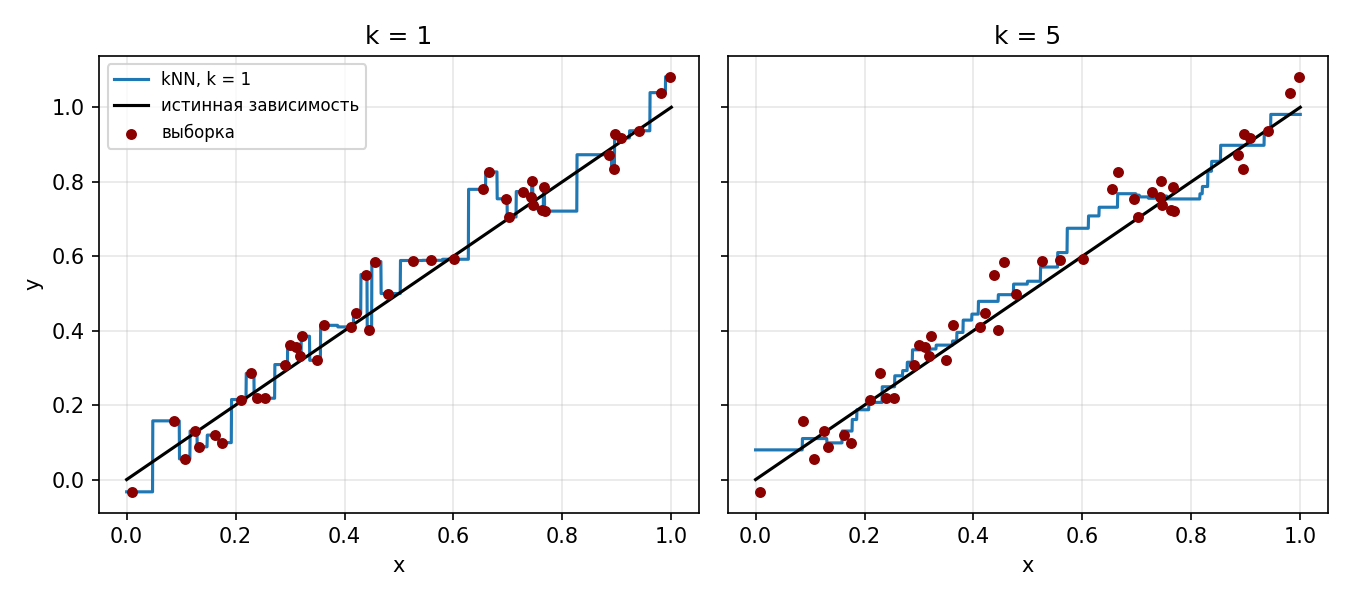
\includegraphics[width=\textwidth]{knn-regression.png}
  \caption{Регрессия методом ближайшего соседа. Слева $k = 1$: ломаная проходит
  через все точки выборки. Справа $k = 5$: ступени стали шире, через точки
  ломаная больше не проходит.}
\end{figure}

\zad{2}
\dano Задача классификации конфигурации потока смеси по вектору признаков
$\xs{i} \in \R^{20}$. Используется классификация по регулярной сетке: диапазон
допустимых значений $[a_j, b_j]$ каждой из компонент делится на $n$ равных
частей, ячейкой называется получившийся многомерный параллелепипед, и объект
относится к тому классу, представителей которого в его ячейке больше. Для
уверенного прогноза требуется $M$ элементов выборки в каждой ячейке.

\treb Найти необходимый размер выборки $N$. Найти $N$ для случая
$\xs{i} \in \R^{40}$.

\resh Каждая из $m$ координат делится на $n$ частей независимо от остальных,
поэтому ячейка однозначно задаётся набором из $m$ номеров подынтервалов, по
одному на координату. Наборов ровно
\[
  \underbrace{n \cdot n \cdot \ldots \cdot n}_{m} = n^m .
\]
Требование $M$ элементов в каждой ячейке даёт
\begin{equation}\label{eq:N}
  N = M\,n^m .
\end{equation}
При $m = 20$ получаем $N = M n^{20}$, при $m = 40$ получаем $N = M n^{40}$.
Удвоение размерности возводит требуемый размер выборки в квадрат:
\[
  N(2m) = M n^{2m} = \frac{(M n^{m})^2}{M} = \frac{N(m)^2}{M} .
\]

Оценка \eqref{eq:N} является нижней: она отвечает идеальному случаю, когда точки
распределены по ячейкам равномерно. Реальные данные распределены неравномерно,
часть ячеек остаётся пустой, и на практике выборка нужна ещё больше.

Подставим правдоподобные значения $n = 10$ и $M = 100$.

\begin{center}
\begin{tabular}{ccc}
\toprule
$m$ & число ячеек $n^m$ & $N = M n^m$ \\
\midrule
$12$ & $10^{12}$ & $10^{14}$ \\
$20$ & $10^{20}$ & $10^{22}$ \\
$40$ & $10^{40}$ & $10^{42}$ \\
\bottomrule
\end{tabular}
\end{center}

Чтобы оценить масштаб: при $m = 20$ одно только хранение выборки потребует
$10^{22}\cdot 20 \cdot 8 = 1.6\cdot10^{24}$ байт, если каждая компонента
занимает восемь байт. Носителей такого объёма не существует, и никакой
эксперимент столько измерений не даст. Процедура, вполне работоспособная при
$m = 2$ или $m = 3$, становится неосуществимой уже при нескольких десятках
признаков.

\zad{3}
\dano Выборка из $N$ элементов, распределённых равномерно в единичном гиперкубе
$[0,1]^m$; по ней требуется оценить плотность распределения.

\treb Показать четыре свойства многомерного куба: (а) почти все точки выборки
лежат у границы; (б) найти длину ребра $l_m(p)$ подкуба, содержащего долю $p$
точек, и оценить $l_5(0.01)$, $l_5(0.1)$, $l_{20}(0.01)$, $l_{20}(0.1)$;
(в) почти все евклидовы расстояния между точками велики и примерно одинаковы, а
окрестность, содержащая хотя бы немного точек, обязана иметь большой радиус;
(г) расстояния Чебышёва между почти всеми точками велики.

\subsection*{а) Точки лежат у границы}

\resh Повторим для куба расчёт \eqref{eq:shell}, сделанный для шара. Точка
удалена от границы не менее чем на $\varepsilon$, если каждая её координата
лежит в $[\varepsilon, 1-\varepsilon]$. Такие точки образуют внутренний куб с
ребром $1 - 2\varepsilon$ и объёмом $(1-2\varepsilon)^m$. При равномерном
распределении вероятность попасть внутрь равна этому объёму, поэтому доля точек
в приграничном слое равна
\[
  1 - (1 - 2\varepsilon)^m \xrightarrow[m \to \infty]{} 1
  \qquad\text{при любом фиксированном } \varepsilon < \tfrac12 .
\]
Сходимость экспоненциальная: при $\varepsilon = 0.05$ доля равна
$1 - 0.9^{20} = 0.878$ для $m = 20$ и $0.995$ для $m = 50$. $\blacksquare$

Содержательно это означает следующее. Если считать, что ошибка измерения
ограничена по каждой координате, то результаты измерений заполняют окрестность
истинного значения. В большой размерности почти все они окажутся не около
истинного значения, а у границы этой окрестности, то есть с ошибкой, близкой к
максимально допустимой сразу по многим координатам.

\subsection*{б) Длина ребра подкуба}

\resh Доля точек, попавших в подкуб, равна его объёму, а объём подкуба с ребром
$l$ равен $l^m$. Из уравнения $l^m = p$ получаем
\begin{equation}\label{eq:edge}
  l_m(p) = p^{1/m} . \qquad\blacksquare
\end{equation}

\begin{center}
\begin{tabular}{ccc}
\toprule
$m$ & $p$ & $l_m(p) = p^{1/m}$ \\
\midrule
$5$  & $0.01$ & $0.3981$ \\
$5$  & $0.1$  & $0.6310$ \\
$20$ & $0.01$ & $0.7943$ \\
$20$ & $0.1$  & $0.8913$ \\
\bottomrule
\end{tabular}
\end{center}

Прочитаем таблицу. Чтобы в $\R^{20}$ собрать всего один процент выборки,
окрестность должна занимать $79\%$ диапазона каждой координаты, а чтобы собрать
десять процентов -- $89\%$. Такая окрестность покрывает почти весь диапазон
изменения каждого признака и локальной не является ни в каком смысле. Метод
ближайшего соседа при этом перестаёт быть локальным методом: усреднение ведётся
по точкам, которые близкими не являются. При $m \to \infty$ величина
$p^{1/m} \to 1$ для любого фиксированного $p > 0$.

\subsection*{в) Евклидовы расстояния}

\resh Пусть $u$ и $v$ -- две независимые точки, равномерные в $[0,1]^m$, и
$d^2 = \sum_{i=1}^{m}(u_i - v_i)^2$. Найдём среднее и дисперсию $d^2$.

Разность двух независимых равномерных на $[0,1]$ величин $w = u_i - v_i$ имеет
треугольную плотность $1 - \abs{w}$ на отрезке $[-1,1]$. Отсюда
\[
  \Exp w^2 = 2\int_0^1 w^2(1-w)\dd w = 2\Bigl(\frac13 - \frac14\Bigr) = \frac16,
\]
\[
  \Exp w^4 = 2\int_0^1 w^4(1-w)\dd w = 2\Bigl(\frac15 - \frac16\Bigr) = \frac{1}{15},
  \qquad
  \Var w^2 = \frac{1}{15} - \frac{1}{36} = \frac{7}{180} .
\]
Слагаемые независимы, поэтому средние и дисперсии складываются:
\[
  \Exp d^2 = \frac{m}{6}, \qquad \Var d^2 = \frac{7m}{180} .
\]
Относительный разброс квадрата расстояния равен
\begin{equation}\label{eq:conc}
  \frac{\sqrt{\Var d^2}}{\Exp d^2}
  = \frac{\sqrt{7m/180}}{m/6}
  = \sqrt{\frac{36 \cdot 7}{180\,m}}
  = \sqrt{\frac{1.4}{m}}
  \xrightarrow[m \to \infty]{} 0 .
\end{equation}
Итак, само расстояние растёт как $\sqrt{m/6}$, а его относительный разброс
убывает как $1/\sqrt{m}$: расстояния становятся большими и почти одинаковыми,
отношение $(d_{\max} - d_{\min})/d_{\min}$ стремится к нулю. Ближайший сосед
почти не отличается по расстоянию от самого далёкого элемента выборки, и понятие
близости обесценивается. $\blacksquare$

Теперь про радиус окрестности. По \eqref{eq:ball} шар радиуса $r$ содержит долю
точек $K_m r^m$, пока он лежит внутри куба, поэтому для доли $p$ нужен радиус
\[
  r = \Bigl(\frac{p}{K_m}\Bigr)^{1/m} .
\]
Величина $K_m = \pi^{m/2}/\Gamma(m/2+1)$ убывает быстрее любой экспоненты, так
что радиус приходится брать всё больший. Предельно наглядный случай: наибольший
шар, вписанный в единичный куб, имеет радиус $1/2$ и объём
\[
  \frac{K_m}{2^m}
  = \frac{\pi^{m/2}}{2^m\,\Gamma(m/2+1)}
  = 2.46\cdot10^{-8} \quad\text{при } m = 20 .
\]
То есть даже самый большой помещающийся в куб шар практически пуст: почти весь
объём куба сосредоточен в его углах, куда шар не достаёт. Любая окрестность,
содержащая заметную долю выборки, обязана выходить за пределы куба.

\subsection*{г) Расстояния Чебышёва}

\resh Расстояние Чебышёва $\rho_\infty = \max_{1\le i\le m}\abs{u_i - v_i}$ не
превосходит $t$ тогда и только тогда, когда по каждой координате расхождение не
превосходит $t$. События по разным координатам независимы, а для треугольной
плотности
\[
  \PP(\abs{w} \le t) = \int_{-t}^{t}(1 - \abs{w})\dd w = 2t - t^2 ,
\]
поэтому
\begin{equation}\label{eq:cheb}
  \PP(\rho_\infty \le t) = (2t - t^2)^m .
\end{equation}
Основание $2t - t^2$ меньше единицы при любом $t < 1$, значит правая часть
стремится к нулю с ростом $m$: почти все чебышёвские расстояния превосходят $t$.
Медиана находится из $ (2t-t^2)^m = 1/2$, то есть $2t - t^2 = 2^{-1/m}$, откуда
\[
  t_{1/2} = 1 - \sqrt{1 - 2^{-1/m}}
  \xrightarrow[m \to \infty]{} 1 .
\]
Численно: $0.640$ при $m = 5$, $0.815$ при $m = 20$, $0.917$ при $m = 100$.
Максимально возможное расстояние Чебышёва в единичном кубе равно единице, то
есть типичное расстояние приближается к максимальному. $\blacksquare$

\smallskip
Все четыре пункта говорят об одном и том же с разных сторон: в пространстве
большой размерности выборка прижимается к границе, локальная окрестность
вынуждена покрывать почти весь диапазон каждого признака, а расстояния между
точками велики и почти одинаковы независимо от выбора нормы. Поэтому
размерность вектора признаков нужно держать минимально достаточной, к чему и
подводит метод главных компонент.

\end{document}
